\chapter{Nonparametric Estimation of Regression and Classification Functions}
\label{chap:nonparregclass}

In some applications, there may be no good parametric model, say linear
or logistic, for $m_{Y;X}$.  Or, we may have a parametric model that we
are considering, but we would like to have some kind of nonparametric
estimation method available as a means of checking the validity of our
parametric model.  So, how do we estimate a regression function
nonparametrically?

Many, many methods have been developed.  We introduce a few here.

\section{Methods Based on Estimating $m_{Y;X}(t)$}

To guide our intuition on this, let's turn again to the example of
estimating the relationship between height and weight.  Consider
estimation of the quantity $m_{W;H}(68.2)$, the {\it population} mean
weight of all people of height 68.2.  

We could take our estimate of $m_{W;H}(68.2)$,
$\widehat{m}_{W;H}(68.2)$,  to be the average weight of all the people
in our sample who have that height.  But we may have very few people of
that height (or even none), so that our estimate may have a high
variance, i.e. may not be very accurate.

What we could do instead is to take the mean weight of all the people in
our sample whose heights are {\it near} 68.2, say between 67.7 and 68.7.
That would bias things a bit, but we'd get a lower variance.  This is
again an illustration of the variance/bias tradeoff introduced in
Section \ref{biasvartradeoff}.

All nonparametric regression/classification (or ``machine learning'')
methods work like this.  There are many variations, but at their core
they all have this same theme.  (Again, note the Hillel quote at the
beginning of Section \ref{meanisprob}.)

As noted earlier, the classification problem is a special case of
regression, so in the following material we will usually not distinguish
between the two.

\subsection{Nearest-Neighbor Methods}

In Chapter\ref{nonpardens}, we presented both kernel and
nearest-neighbors for density estimation.  The same two approaches can
be used to estimate regression functions.  

In the {\bf nearest-neighbor} approach, we for instance estimating
$m_{Y;X}(68.2)$ to be the mean weight of the k people in our sample with
heights nearest 68.2.  Here k controls bias/variance tradeoff.

Note that if we have more than one predictor variable, the
distance used to determine ``nearest'' is multivariate, e.g. the
distance in the plane in the case of two predictors.

In spite of the apparently simple notion here, nearest-neighbor
regression and classification methods are quite effective and popular.
Several contributed packages on the CRAN site for R implement this idea.

Here is simple (nonoptimized) code to do all this:

\begin{lstlisting}[numbers=left]
# the function knn() does k-nearest neighbor regression; the user has a
# choice of either just fitting to the x,y dataset or using that data to
# predict new observations newobs for which only the predictors are
# known

# arguments:

# x:  matrix or data frame of the predictor variable data, one row per
#     observation
#
# y:  vector of the response variables corresponding to x; in the
#     classification case, these are assumed to be 1s and 0s
#
# k:  the number of nearest neighbors to use for estimating the regression
#     or predicting the new data
#
# newobs:  a matrix of values of the predictors, one row per observation,
#          on which to predict the responses; default value is NULL
#
# regtype:  "reg" for prediction of continuous variables, "cls" for
#           classification problems; default value "reg"
#

# return value: an R list with the following components
#
#    regvals:  estimated values of the regression function at x
#
#    predvals:  if newobs is not NULL, predicted values for y from newobs
#               otherwise NULL
#
#    predsuccess:  if newobs is NULL, then R^2 in the "reg" case, proportion 
#                  of correctly classified observations in the "cls" case; 
#                  otherwise NULL

library(RANN)  # fast nearest-neighbor finder on CRAN

knn <- function(x,y,k,newobs=NULL,regtype="reg") {
   # make sure x is a matrix or data frame for use with RANN
   if (is.vector(x)) x <- matrix(x,ncol=1)
   retval <- list()
   # just trying out on current data set?
   if (is.null(newobs)) {
      nearones <- nn2(data=x,k=k,query=x)$nn.idx
   } else {
      nearones <- nn2(data=x,k=k,query=newobs)$nn.idx
   }
   # row i of nearones now consists of the indices in x of the k closest
   # observations in x to row i of x or row i of newobs
   #
   # now find the estimated regression function at each row
   regvals <- apply(nearones,1,pred1y,y)
   if (is.null(newobs)) {
      if (regtype=="reg") {
         tmp <- cor(regvals,y)
         predsuccess <- tmp^2
      } else {
         predvals <- as.integer(regvals > 0.5)
         predsuccess <- mean(predvals == y)
      }
      predvals <- NULL
   } else {
      predsuccess <- NULL 
      newregvals <- apply(nearones,1,pred1y,y)
      if (regtype == "reg") predvals <- newregvals else {
         predvals <- as.integer(regvals > 0.5)  
      }
   }
   retval$regvals <- regvals
   retval$predvals <- predvals
   retval$predsuccess <- predsuccess
   retval
}

# for a single observation, calculate the value of the regression
# function there, knowing the indices xidxs of the values in the
# original data x that are closest to the given observation
pred1y <- function(xidxs,y) predval <- mean(y[xidxs])

\end{lstlisting}

\subsection{Kernel-Based Methods}

As our definition of ``near,'' we could take all people in our sample
whose heights are within h amount of 68.2.  This should remind you of
our density estimators in Chapter \ref{chap:nonpardens}.  A
generalization would be to use a {\bf kernel} method.  For instance, for
univariate X and t:

\begin{equation}
\widehat{m}_{Y;X}(t) = \frac
{\sum_{i=1}^{n} Y_i k\left ( \frac{t-X_i}{h}   \right ) }
{\sum_{i=1}^{n} k\left ( \frac{t-X_i}{h}   \right ) }
\end{equation}

Again note that if we have more than one predictor variable, the
function k() has a multivariate argument.

Here k() is a density, i.e. a nonnegative function that integrates to 1.
Also, it is almost always chosen so that k() is symmetric around 0, with
a peak at 0 and then tapering off as one moves away from 0 in either
direction.

This looks imposing!  But it is simply a weighted average of the Y values
in our sample, with the larger weights being placed on observations for
which X is close to t.  

Note the word {\it chosen}.  The analyst makes this choice (or takes a
default value, say in an R library), simply from considerations of
weighting: Choosing k() to be a ``tall, narrow'' function will make the
weights drop off more rapidly to 0.

In fact, the choice of kernel is not very important (often it is taken
to be the N(0,1) density.)  What does matter is the parameter h.  The
smaller h is, the more our weighting will concentrate on nearby
observations.

In other words, setting a smaller value of h is quite analogous to
choosing a smaller value of k (the number of nearest neighbors, not our
kernel function here) in nearest-neighbor regression.

As before, the choice of h here involves a bias/variance tradeoff.  We
might try choosing h via cross validation, as discussed in Section
\ref{varsel}.

There is an R package that includes a function {\bf nkreg()} for kernel
regression.  The R base has a similar method, called {\bf LOESS}.  Note:
That is the class name, but the R function is called {\bf lowess()}.

\subsection{The Naive Bayes Method}

This method is for the classification problem only.

The Naive Bayes method is not ``Bayesian'' in the sense of Section
\ref{bayesian}.  Instead, its name comes simply from its usage of Bayes'
Rule for conditional probability.  It basically makes the same
computations as in Section \ref{logitmotivations}, for the case in which
the predictors are indicator variables and are independent of each
other, given the class.  

The term {\it naive} is an allusion to analysts who naively assume
independent predictors, without realizing that they are making a serious
restriction.

Under that assumption, the numerator in (\ref{intermedone}) becomes

\begin{equation}
P(Y = 1) ~~ P[X^{(1)}=t_1|Y=1]~~ ...~~ P[X^{(r)}=t_r|Y=1]
\end{equation}

All of those quantities (and similarly, those in the denominator of
(\ref{intermedone}) can be estimated directly as sample proportions.
For example, $\widehat{P}[X^{(1)}=t_1|Y=1]$ would be the fraction of
$X_j^{(1)}$ that are equal to $t_1$, among those observations for which
$Y_j = 1$.

A common example of the use of Naive Bayes is text mining, as in Section
\ref{textmining}.  Our independence assumption in this case means that
the probability that, for instance, a document of a certain class
contains both of the words {\it baseball} and {\it strike} is the
product of the individual probabilities of those words.

Clearly the independence assumption is not justified in this
application.  But if our vocabulary is large, that assumption limits the
complexity of our model, which may be necessary from a bias/variance
tradeoff point of view (Section \ref{biasvartradeoff}).  

\section{Methods Based on Estimating Classification Boundaries}

In the methods presented above, we are estimating the function
$m_{Y;X}(t)$.  But with support vector machines and CART below, we are
in a way working backwards.  In the classification case (which is what
we will focus on), for instance, our goal is to estimate the values of t
for which the regression function equals 0.5:

\begin{equation}
\label{boundary}
B = \{t: m_{Y;X}(t) = 0.5\}
\end{equation}

Recall that r is the number of predictor variables we have.  Then note
the geometric form that the set B in (\ref{boundary}) will take on:
discrete points if r = 1; a curve if r = 2; a surface if r = 3; and a
hypersurface if r $>$ 3.

The motivation for using (\ref{boundary}) stems from the fact, noted in
Section \ref{meanisprob}, that if we know $m_{Y;X}(t)$, we will predict
Y to be 1 if and only if $m_{Y;X}(t) > 0.5$.  Since (\ref{boundary})
represents the boundary between the portions of the X space for which
$m_{Y;X}(t)$ is either larger or smaller than 0.5, it is the boundary
for our prediction rule, i.e. the boundary separating the regions in X
space in which we predict Y to be 1 or 0.

Lest this become too abstract, again consider the simple example of
predicting gender from height and weight.  Consider the (u,v) plane,
with u and v representing height and weight, respectively.  Then
(\ref{boundary}) is some curve in that plane.  If a person's
(height,weight) pair is on one side of the curve, we guess that the
person is male, and otherwise guess female.

If the logistic model (\ref{logit2}) holds, then that curve is actually
a straight line.  To see this, note that in (\ref{logit2}), the equation
(\ref{boundary}) boils down to 

\begin{equation}
\label{logit0}
\beta_0+\beta_1 u + \beta_2 v = 0
\end{equation}

whose geometric form is a straight line.

\subsection{Support Vector Machines (SVMs)}

This method has been getting a lot of publicity in computer science
circles (maybe too much; see below).  It is better explained for the
classification case.

In the form of dot product (or inner product) from linear algebra,
(\ref{logit0}) is

\begin{equation}
\label{dotprod}
(\beta_1, \beta_2)' (u,v) = -\beta_0
\end{equation}

What SVM does is to generalize this, for instance changing the criterion
to, say

\begin{equation}
\label{kernel2}
\beta_0 u^2 + \beta_1 uv + \beta_2 v^2 + \beta_3 u + \beta_4 v = 1
\end{equation}

Now our $(u,v)$ plane is divided by a curve instead of by a straight
line (though it includes straight lines as special cases), thus
providing more flexibility and thus potentially better accuracy.

In SVM terminology, (\ref{kernel2}) uses a different {\bf kernel} than
regular dot product.  (This of course should not be confused our the
term {\it kernel} in kernel-based regression above.)  The actual method
is more complicated than this, involving transforming the original
predictor variables and then using an ordinary inner product in the
transformed space.  In the above example, the transformation consists of
squaring and multiplying our variables.  That takes us from
two-dimensional space (just u and v) to five dimensions ($u$, $v$,
$u^2$, $v^2$ and $uv$).

There are various other details that we've omitted here, but the essence
of the method is as shown above.

Of course, a good choice of the kernel is crucial to the successful
usage of this method.  It is the analog of h and k in the nearness-based
methods above.

A former UCD professor, Nello Cristiani, is one of the world leaders in
SVM research.  See {\it An Introduction to Support Vector Machines}, N.
Cristianini and J. Shawe-Taylor, Cambridge University Press, 2000.

\subsection{CART}

Another nonparametric method is that of {\bf Classification and
Regression Trees} (CART).  It's again easiest explained in the
classification context, say the diabetes example above.

In the diabetes example, we might try to use glucose variable as our
first predictor.  The data may show that a high glucose value implies a
high likelihood of developing diabetes, while a low value does the
opposite.  We would then find a {\bf split} on this variable, meaning a
a cutoff value that defines ``high'' and ``low.''  Pictorially, we draw
this as the root of a tree, with the left branch indicating a tentative
guess of no diabetes and the right branch corresponding to a guess of
diabetes.

Actually, we could do this for all our predictor variables, and find
which one produces the best split at the root stage.  But let's assume
that we find that glucose is that variable.

Now we repeat the process.  For the left branch---all the subset of our
data corresponding to ``low'' glucose---we find the variable that best
splits that branch, say body mass index.  We do the same for the right
branch, say finding that age gives the best split.  We keep going until
the resulting cells are too small for a reasonable split.

An example with real data is given in a tutorial on the use of {\bf
rpart}, an R package that does analysis of the CART type, {\it An
Introduction to Recursive Partitioning Using the RPART Routines}, by
Terry Therneau and Elizabeth Atkinson.  The data was on treatment of
cardiac arrest patients by emergency medical technicians.

The response variable here is whether the technicians were able to
revive the patient, with predictors $X^{(1)}$ = initial heart rhythm,
$X^{(2)}$ = initial response to defrillabration, and $X^{(3)}$ = initial
response to drugs.  The resulting tree was

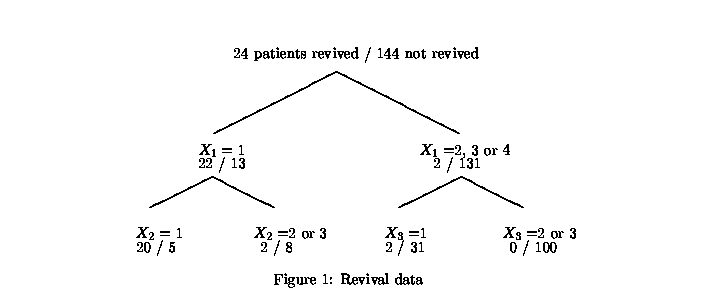
\includegraphics[width=7.0in]{RPart.jpg}

So, if for example a patient has $X^{(1)}=1$ and $X^{(2)} = 3$, we would
guess him to be revivable.

CART is a boundary method, as SVM is.  Say for instance we have two
variables, represented graphically by s and t, and our root node rule is
$s > 0.62$.  In the left branch, the rule is $t > 0.8$ and in the right
branch it's $t > 0.58$.  This boils down to a boundary line as follows:

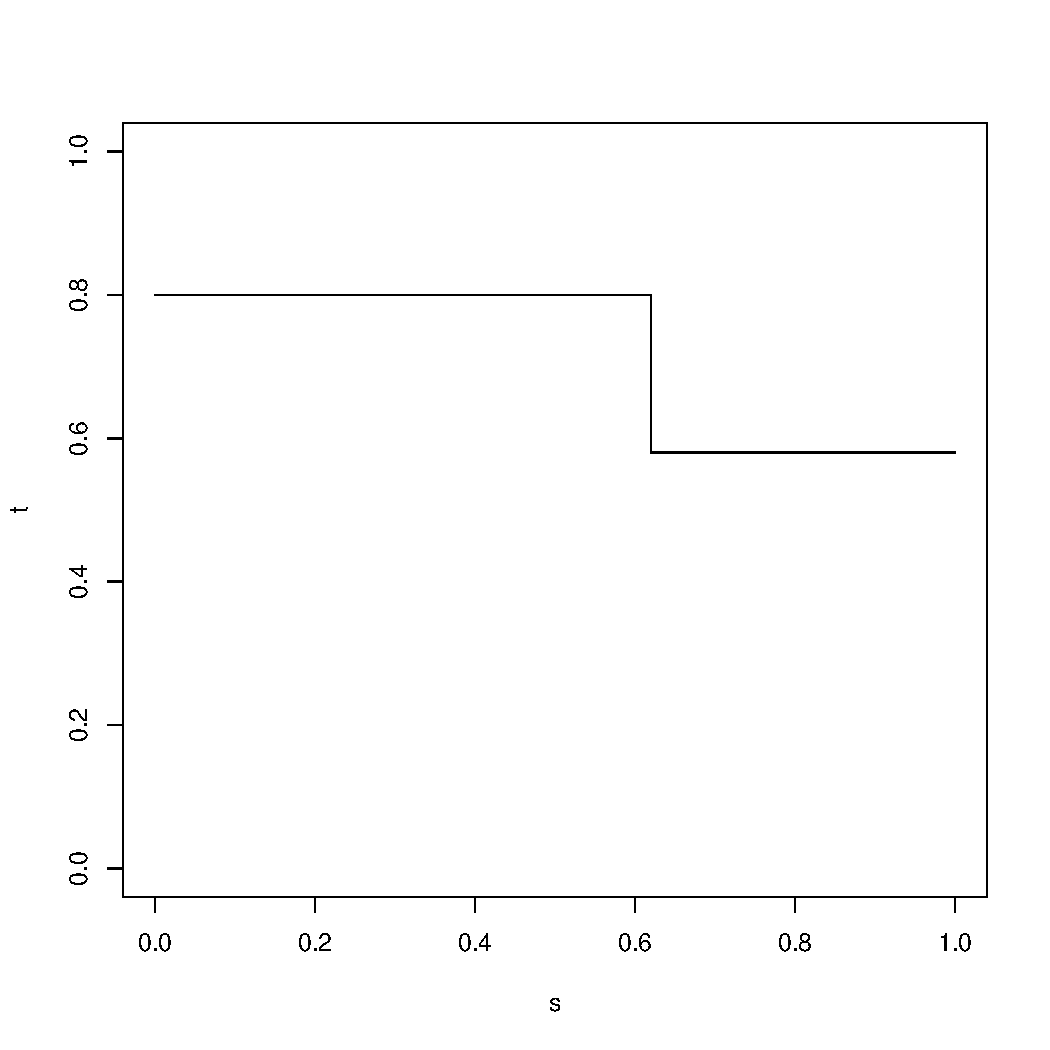
\includegraphics[width=5.0in]{CARTBound.pdf}

CART obviously has an intuitive appeal, easily explained to
nonstatisticians, and easy quite easy to implement.  It also has the
virtue of working equally well with discrete or continuous predictor
variables.

The analogs here of the h in the kernel method and k in nearest-neighbor
regression are the choice of where to define the splits, and when to stop
splitting.  Cross validation is often used for making such decisions.

\section{Comparison of Methods}

{\bf Beware!  There are no ``magic'' solutions to statistical problems.}
The statements one sees by some computer science researchers to the
effect that SVMs are generally superior to other prediction methods are,
unfortunately, unfounded; there just is no generally superior method.  

First, note that every one of the above methods involves some choice of
tuning parameter, such as h in the kernel method, k in the
nearest-neighbor method, the split points in CART, and in the case of
SVM, the form of kernel to use.  For SVM the choice of kernel is
crucial, yet difficult.

Second, the comparisons are often unfair, notably comparisons of the
logit model to SVM.  Such comparisons usually limit the logit
experiments to first-degree terms without interactions.  But the kernel
in SVM is essentially analogous to throwing in second-degree and
interaction terms, and so oni, (\ref{logit2}) for the logit case, thus
producing a curved partitioning line just like SVM does.

I highly recommend the site \url{www.dtreg.com/benchmarks.htm}, which
compares six different types of classification function
estimators---including logistic regression and SVM---on several dozen
real data sets.  The overall percent misclassification rates, averaged
over all the data sets, was fairly close, ranging from a high of 25.3\%
to a low of 19.2\%.  The much-vaunted SVM came in at an overall score
across all data sets of 20.3\%.  That's nice, but it was only a tad
better than logit's 20.9\%---and remember, that's with logit running
under the handicap of having only first-degree terms.

Or consider the annual KDDCup competition, in which teams from around
the world compete to solve a given classification problem with the
lowest misclassification rate.  In KDDCup2009, for instance, none of the
top teams used SVM.  See {\it SIGKDD Explorations}, December 2009 issue.

Considering that logit has a big advantage in that one gets an actual
equation for the classification function, complete with parameters which
we can estimate and make confidence intervals for, it is not clear just
what role SVM and the other nonparametric estimators should play, in
general, though in specific applications they may be appropriate.

